\section{Kennenlernen von AWS}
\section{Kanban}\label{appendix:kanban}
\begin{figure}[H]
	\centering
	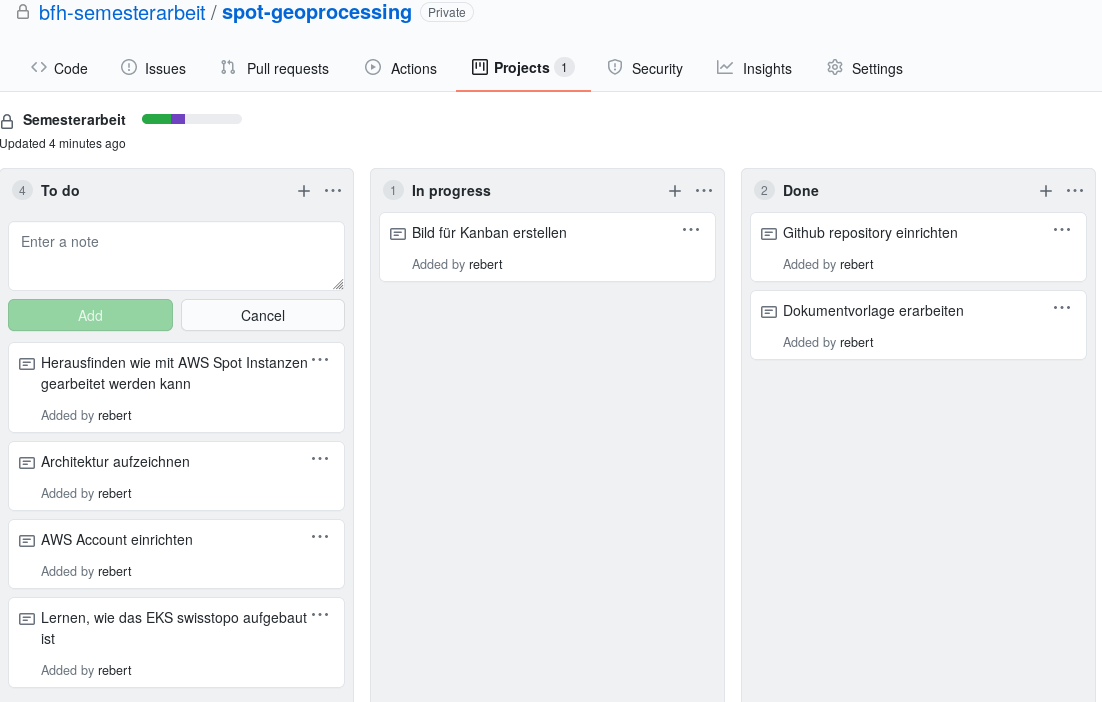
\includegraphics[width=.95\textwidth]{kanban}
	\caption{Klassisches Kanban auf \emph{github.com}}
	\label{fig:Klassisches Kanban}
\end{figure}

\section{Projektplan}\label{appendix:projektplan}
\begin{figure}[H]
	\centering
	\href{https://docs.google.com/spreadsheets/d/1zKTZgt4BW736G0xRfU9o3vWYwAJj-8nzFvGsPR7yJ_0/edit?usp=sharing}{
	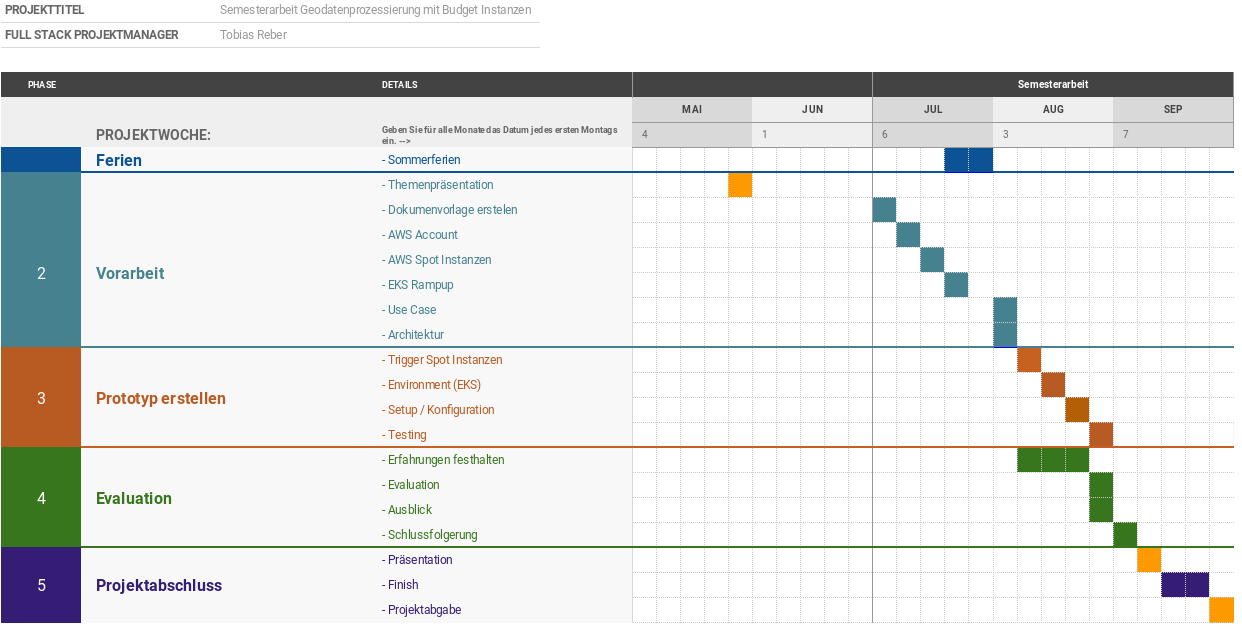
\includegraphics[width=.95\textwidth]{projektplanung}}
	\caption{\href{https://docs.google.com/spreadsheets/d/1zKTZgt4BW736G0xRfU9o3vWYwAJj-8nzFvGsPR7yJ_0/edit?usp=sharing}{Projektplan. Die orangen Meilensteine wurden von der BFH vorgegeben.}}
	\label{fig:Projektplan}
\end{figure}

\section{Konfigurationen und Kommandos}
\subsection{XML Testen}
Einfaches Skript, um zu testen, ob alle XML-Dateien well-formed sind.
\appendCode{python}{XML testen}{src/up-and-running-dataprocessing/ansible/tests/test_xml_wellformed.py}

\subsection{EFS auf EC2-Instanz mounten}
Anhand einer Anleitung, einem sogenannten Walktrough, wurde via AWS CLI\footnote{AWS Command Line Interface: Ein kommandozeilenorientiertes Werkzeug.} ein
EFS an eine EC2-Instanz gemountet und die 3D Daten wurden dorthin kopiert.
\appendCode{bash}{EFS auf EC2-Instanz mounten}{src/walktrough_ec2_and_efs.sh}

\subsection{Von der SPOT Instanz aus abfragen, was ihr Status ist}\label{appendix:restful}
Von der Instanz aus können via RESTful API Metadaten der Instanz abgefragt werden. Bezüglich Determinierung einer Spot-Instanz kann der Zustand \emph{none}, \emph{hibernate}, \emph{stop} oder \emph{terminate} sein. \emph{none}, wenn nichts ansteht. Von da an, wo klar ist, dass die Instanz abgestellt werden wird, kann der Zeitpunkt ausgelesen werden.
\appendCode{bash}{Status der Instanz abfragen}{src/rest_instance_metadata.sh}

\section{Für die Semesterarbeit verwendete Software}
\begin{itemize}
\item JabRef: Verwaltung des Literaturverzeichnisses (BibTeX).
\item Gummi: LaTeX Editor.
\item AWS CLI: Für das Bereitstellen der AWS Infrastruktur.
\item jq: Für das Filtern von JSON (vor allem von AWS CLI Antworten).
\item git: Versionsmanagement der Textdateien.
\item Google Spreadsheet: Für den \nameref{chap:projektplan}.
\end{itemize}
